%%
%% $Id$
%%
%% Copyright (c) 2007-2008 Christian Fehler
%% Copyright (c) 2007-2008 Benjamin Mies
%%


\chapter{Konvertierung}\label{ConverTo}

In diesem Kapitel soll das Umwandeln von einer Grammatik in einen Automaten bzw.
zwischen den verschiedenen Automatentypen besprochen werden. Dabei wird im
Besonderen darauf eingegangen, welche Herausforderungen aufgetreten sind, um dem
Benutzer die verwendeten Algorithmen möglichst in kleinen Schritten darzustellen.
Beim Umwandeln von Grammatiken in die entsprechenden Automaten sind die
verwendeten Algorithmen leicht zu verstehen und nicht besonders gut darzustellen,
weshalb hier darauf verzichtet wurde, dem Benutzer eine schrittweise Umwandlung
anhand einer graphischen Darstellung zu präsentieren.\vspace{10pt}


\section{Grammatik Konvertierung}\label{ConverToGrammar}

Wenn ein Benutzer eine Grammatik vollständig erstellt hat, kann es durchaus
interessant sein, den Automaten zu sehen, welcher die Sprache akzeptiert, die
durch die Grammatik beschrieben wird. Vor allem, da für Automaten weitaus mehr
Verwendungsmöglichkeiten in diesem Werkzeug existieren.\vspace{10pt}

\subsection{Konvertierung einer regulären Grammatik}\label{ConverToGrammarRegular}

%### removes texlipse warning
Eine reguläre Grammatik kann in einen entsprechenden nicht deterministischen,
endlichen Automaten umgewandelt werden. Der verwendete Algorithmus kann in
\cite{Compilers} nachgelesen werden. Die Zustände unseres entstehenden Automaten
resultieren aus den Nichtterminalzeichen unserer Grammatik. Allerdings werden in
der Implementierung nur Zustände für die Nichtterminalzeichen angelegt, welche
auch in einer Produktion, auf der rechten oder linken Seite, verwendet werden.
Die Zustände werden immer dann angelegt, wenn man auf ein Nichtterminalzeichen
trifft, welches man bis jetzt noch nicht gesehen hat.\vspace{10pt}
%### removes texlipse warning

Die rechte Seite einer Produktion kann entweder aus einem einzelnen
Terminalzeichen ($\NonterminalSymbol{S} \to \TerminalSymbol{a}$), oder
aus einem Terminalzeichen mit einem anschließenden Nichtterminalzeichen
($\NonterminalSymbol{S} \to \TerminalSymbol{a}\NonterminalSymbol{A}$) bestehen,
da nur solche Arten von Produktionen zugelassen sind.\vspace{10pt}

Am Anfang legen wir einen akzeptierenden Zustand an, welchen wir im weitern
Verlauf des Algorithmus noch benötigen werden.\vspace{10pt}

 Wir betrachten der Reihe nach
jede Produktion der Grammatik. Zunächst interessiert uns die linke Seite. Wenn wir das Nichtterminalzeichen
bereits gesehen haben, wurde auch schon ein Zustand dafür angelegt, und wir
merken uns diesen. Wenn wir das Nichtterminalzeichen noch nicht gesehen haben,
müssen wir jetzt einen neuen Zustand anlegen, welcher dieses repräsentiert, und
merken uns diesen neuen Zustand, da dieser der Ausgangszustand
für die zu erstellenden Übergänge ist.\vspace{10pt}

Als nächstes betrachten wir die rechte Seite der Produktion. Wenn es sich dabei
um ein einzelnes Terminalzeichen handelt, wird ein Übergang von dem Zustand für
das Nichtterminalzeichen zu dem akzeptierenden Zustand erzeugt, wobei die
Übergangsmenge aus dem Terminalzeichen auf der rechten Seite der Produktion
besteht.\vspace{10pt}

Besteht die rechte Seite allerdings aus einem Terminalzeichen und einem
Nichtterminalzeichen müssen wir wieder überprüfen, ob wir das
Nichtterminalzeichen bereits gesehen haben, um gegebenenfalls den
entsprechenden Zustand anzulegen. Im nächsten Schritt wird ein Übergang,
zwischen den beiden Zuständen die wir uns gemerkt haben, angelegt, mit der der
rechten Seite der Produktion als Übergangsmenge.\vspace{10pt}

Diese Behandlung wiederholen wir für jede Produktion der Grammatik und
erhalten so einen endlichen Automaten, der genau die von der
Grammatik erzeugte Sprache akzeptiert.\vspace{10pt}

\subsection{a einer kontextfreien
Grammatik}\label{ConverToGrammarContextFree}

%### removes texlipse warning
Der Benutzer hat auch die Möglichkeit, eine zuvor erstellte kontextfreie
Grammatik in einen Kellerautomaten umwandeln zu lassen. Dieser
Algorithmus ist in \cite{Compilers} beschrieben\vspace{10pt}
%### removes texlipse warning

Zu Beginn werden zwei Zustände angelegt, ein Startzustand und ein
akzeptierender Zustand. Dazu wird ein Übergang vom Startzustand in den
akzeptierenden Zustand angelegt, welcher das Startsymbol der Grammatik in den
Keller legt. Dann wird für jede Produktion ein Übergang angelegt, welcher die rechte
Seite der Produktion vom Keller entfernt, und dafür die linke Seite der
Produktion auf den Keller schreibt. Dieser Übergang hat als
Ursprungs- und Zielzustand den akzeptierenden Zustand.\vspace{10pt}

Wenn alle Produktionen verarbeitet wurden, wird zusätzlich pro Terminalzeichen
ein Übergang vom akzeptierenden Zustand in den akzeptierenden Zustand angelegt.
In jedem dieser Übergänge wird das entsprechende Terminalzeichen vom Eingabewort
gelesen und vom Keller des Automaten genommen. Das bedeutet, es muss das gleiche
Terminalzeichen als oberstes im Keller  und als nächstes Zeichen im Wort
stehen.\vspace{10pt}

Durch die Zweite Ansicht (siehe Kapitel \ref{SecondView}) hat der Benuzter auch
die Möglichkeit, die Ausgangsgrammatik und den enstandenen Automaten
nebeneinander zu sehen, um die Zusammenhänge besser verstehen zu können.\vspace{10pt}


\section{Automaten Konvertierung}\label{ConverToMachine}

Bei der Planung der Umwandlung zwischen den verschiedenen Automatentypen stellte
sich die Frage, wie dem Benutzer der Umwandlungsalgorithmus möglichst
verständlich dargestellt wird. Wir entschieden uns für das auch sonst im \gtitool
verwendete Verfahren, eine Navigationsleiste zu verwenden, die es dem Benutzer
gestattet, in dem Algorithmus einen Schritt vor bzw. einen Schritt zurück zu
gehen. Um die Handhabung für den Benutzer zu erleichtern, wurde die
Navigationsleiste so erweitert, dass der Benutzer sowohl zurück an den Anfang der
Ausführung des Algorithmus springen kann, als auch an das Ende. Des weiteren
sollten die einzelnen Schritte auch automatisch, nach einer einstellbaren Zeit,
durchgeführt werden können.\vspace{10pt}

Um dem Benutzer den durchgeführten Algorithmus zu verdeutlichen, wurde die
Ansicht in drei Bereiche eingeteilt. In dem oberen linken Bereich wird der
Ausgangsautomat dargestellt, im unteren linken Bereich der nach und nach
entstehende konvertierte Automat und schließlich im rechten Bereich eine Outline,
die pro Ausführungsphase, jeweils mit einem Kommentar, angibt, welchen Schritt
der Algorithmus im Moment durchführt.\vspace{10pt}

\begin{figure}[h!]
\begin{center}
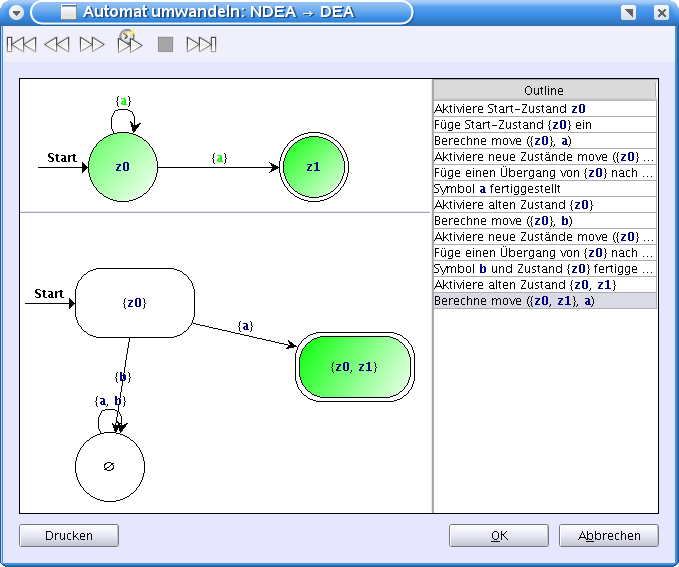
\includegraphics[width=12cm]{../images/convert_to.png}
\caption{Automat umwandeln}
\end{center}
\end{figure}
\vspace{10pt}

Es existieren zwei verschiedene Verfahren zur Umwandlung eines nicht
deterministischen endlichen Automaten in einen deterministischen endlichen
Automaten (DEA). Zum einen kann der komplette Potenzautomat verwendet werden, um
den DEA zu erzeugen. Der entstehende Automat enthält allerdings unter Umständen
sehr viele nicht erreichbare Zustände, deren Berechnung einige zusätzliche
Schritte zur Folge haben kann. Wenn der Benutzer diese Art der Umwandlung
auswählt, kann er nach dem Umwandeln die nicht erreichbaren Zustände wieder
entfernen. Wie dies funktioniert, kann in \ref{ReachableStates} nachgelesen
werden. Die zweite Methode ist, dass nur die erreichbaren Zustände in der unteren
Ansicht angelegt werden. Diese Methode ist übersichtlicher für den Benutzer, wenn
auch nicht alle im Potenzautomaten vorhandenen Zustände betrachtet
werden.\vspace{10pt}

\newpage
%### removes texlipse warning
Zur Umsetzung wurde der in \cite[S. 153ff]{Compilers} angegebene Algorithmus als
Vorlage benutzt. Um den Algorithmus verstehen zu können, müssen zuerst einige
Terme definiert werden.\vspace{10pt}
%### removes texlipse warning

\noindent
\begin{tabular}{|p{2.2cm}|p{9.0cm}|}
  \hline
  NFA A                 & Input NFA \\
  \hline
  DFA D                 & Output DFA \\
  \hline
  Dstates               & States of output DFA D \\
  \hline
  Dtran                 & Transition function of DFA D \\
  \hline
  $\epsilon$-closure(s) & Set of NFA states reachable from NFA state s
                          on $\epsilon$-transitions alone \\
  \hline
  $\epsilon$-closure(T) & Set of NFA states reachable from some NFA state s
                          in set T on $\epsilon$-transitions alone; =
                          $\cup_{s\ in\ T}\ \epsilon$-closure(s). \\
  \hline
  move(T,a)             & Set of NFA states to which there is a transition
                          on input symbol a from some state s in T \\
  \hline
\end{tabular}
\vspace{10pt}

Die eigentliche Umwandlung geschieht dann mit folgendem Algorithmus, der aus
didaktischen Gründen in mehrere Schritte aufgeteilt wurde.\vspace{10pt}

\noindent
\verb| 1 initially, |$\epsilon$\verb|-closure(|$s_0$\verb|) is the only state in Dstates,|\\
\verb| 2 and it is unmarked;|\\
\verb| 3 while ( there is an unmarked state T in Dstates ) {|\\
\verb| 4       mark T;|\\
\verb| 5       for ( each input symbol a ) {|\\
\verb| 6           U = |$\epsilon$\verb|-closure(move(T,a));|\\
\verb| 7           if ( U is not in Dstates )|\\
\verb| 8              add U as an unmarked state to Dstates;|\\
\verb| 9           Dtran[T,a] = U;|\\
\verb|10       }|\\
\verb|11 }|
\vspace{10pt}
